% Chapter 4
% Roberto Masocco <robmasocco@gmail.com>
% October 8, 2021

\chapter[Controllori e middleware]{Controllori e middleware}
\label{chap:Chapter4} 
\doublespacing
\fontsize{12}{12}\selectfont
\newsection{Premessa}
\indent Nel Capitolo \ref{chap:Chapter3} è stata discussa l'implementazione di un'architettura di controllo basata sul middleware ROS 2. Su tale architettura sono state realizzate le logiche di controllo e supervisione di livello medio-alto del drone autonomo presentato come caso di studio. L'obiettivo di questo capitolo è presentare uno studio preliminare delle possibilità di tale architettura in contesti di più basso livello, relativi ai sistemi di controllo veloci. Verrà dunque proposto un controllore relativo allo stesso caso di studio precedente e che sarà realizzato tramite moduli ROS 2 ed infine testato usando il modello del drone simulato in Gazebo.

\newsection{Problema di controllo}
\indent Il precision landing è una fase critica della missione: dal suo corretto svolgimento dipende l'assegnazione del punteggio relativo alla piazzola su cui lo si esegue. Qualunque disturbo presente in fase di allineamento e discesa, se non correttamente reiezionato, può compromettere la stabilità del volo e dunque la precisione dell'atterraggio sul target. Il problema di controllo che verrà ora studiato è quello del precision landing in presenza di vento. Quest'ultimo è inteso come un disturbo costante di ampiezza e segno non noti a priori, che va a sommarsi alla velocità assunta dal drone mediante il suo sistema di controllo veloce illustrato precedentemente. Si assume inoltre che, per effettuare la procedura con la massima precisione possibile, il drone sia controllato in velocità lineare mediante invio di setpoint appositi, calcolati da un opportuno controllore il cui ingresso sia un segnale d'errore di posizionamento rispetto al target, espresso in metri e campionato dalla camera inferiore a 20 Hz grazie ad uno dei moduli precedentemente descritti. Tale soluzione si configura dunque come un'alternativa rispetto a quella presentata nel Capitolo \ref{chap:Chapter3} e implementata nel modulo Land Corrector, che era basata su una correzione del posizionamento richiesta direttamente al controllo di posizione di PX4. Per semplicità verranno controllati separatamente i posizionamenti lungo gli assi $x$ ed $y$ del sistema di riferimento solidale al suolo, mentre la quota verrà progressivamente abbassata fintantoché l'allineamento sarà corretto secondo la stessa logica del modulo originale, e sempre mediante un controllo in velocità proporzionale alla differenza tra la quota corrente ed il nuovo riferimento. Tale semplice controllo sull'asse $z$ si è dimostrato avere buone performance e pertanto è stato mantenuto.

\newsection{Identificazione del sistema da controllare}
\indent Il problema descritto poc'anzi richiede un'analisi preliminare del sistema da porre sotto controllo: si tratta infatti di una situazione non-standard. Si vuole, in sintesi, controllare il drone, già sotto il controllo stabilizzante del Pixhawk, impostando un riferimento di velocità da fargli inseguire, mediante delle azioni di controllo realizzate dai motori che sono però calcolate da PX4 e supposte ignote. Nonostante l'ipotesi semplificativa di separare il controllo sui due assi, è necessario identificare due diversi sistemi, che esprimano il modo in cui il drone stabilizzato insegue riferimenti di velocità su ciascun asse. Tali sistemi saranno chiaramente nonlineari nella realtà, ma ai fini di questo lavoro è stata giudicata sufficiente una loro approssimazione con modelli lineari di ordine opportuno.\\
La fase di raccolta dati è stata eseguita su Gazebo, impiegando il modulo Flight Control per controllare il drone e definendo delle routine di test per ciascun asse che consistevano nell'invio di diversi setpoint di velocità da inseguire, implementate come script di shell. Durante i voli di prova sono stati registrati tramite bagging i dati di input/output su cui lavorare, nella forma di setpoint correnti e velocità misurate da EKF2 ad ogni istante: i primi inviati dal nodo flight\_controller a 20 Hz sul topic /TrajectorySetpoint e le seconde trasmesse da PX4 sul topic /VehicleOdometry a 100 Hz. Successivamente un nodo ROS 2 scritto ad-hoc ha consentito di ricampionare entrambi i segnali allo stesso rate dell'odometria, dunque 100 Hz, salvandoli infine tutti in un file CSV. I datasets così ottenuti sono mostrati nelle Figure \ref{fig:xdataset} e \ref{fig:ydataset}. Da essi si evince chiaramente come si tratti, in entrambi i casi, di sistemi approssimabili linearmente al primo ordine.\\
La procedura d'identificazione è stata eseguita con l'ausilio della System Identification Toolbox\footnote{https://it.mathworks.com/products/sysid.html} di MATLAB. Il Toolbox è stato impiegato in entrambi i casi per identificare la rappresentazione nello spazio di stato di un sistema lineare del primo ordine usando la \emph{Prediction Error Minimization}, da cui calcolare poi una funzione di trasferimento. I dataset sono stati divisi in due parti, usate rispettivamente per la stima e la validazione. Un confronto tra i modelli approssimati e quelli reali eseguito sui validation sets, unitamente agli intervalli di confidenza, è disponibile nelle Figure \ref{fig:xvalerr} e \ref{fig:yvalerr}, mentre le due funzioni di trasferimento ad essi corrispondenti sono:
\begin{subequations}
    \begin{align}
        W_x(s) &= \frac{1}{s+1.2775}\\
        W_y(s) &= \frac{1}{s+1.4350}
    \end{align}
\end{subequations}
i cui guadagni statici sono stati approssimati pari ad 1 in quanto il controllore di volo insegue i riferimenti di velocità in modo da annullare l'errore a regime.

\begin{figure}
    \centering
    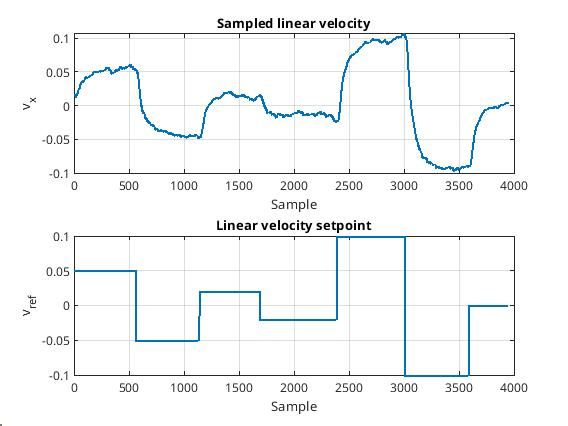
\includegraphics[width=0.8\textwidth]{figs/chapter4/xdataset.jpg}
    \caption{Dataset I/O relativo all'asse $x$.}
    \label{fig:xdataset}
\end{figure}

\begin{figure}
    \centering
    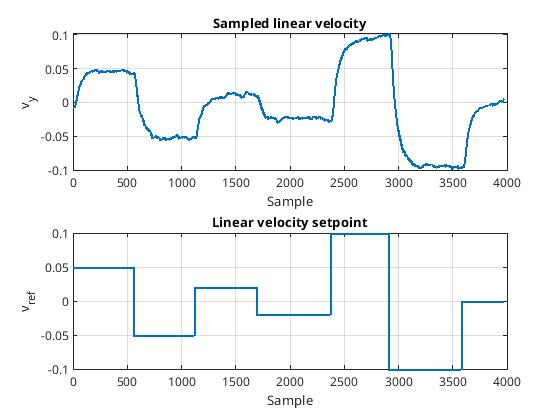
\includegraphics[width=0.8\textwidth]{figs/chapter4/ydataset.jpg}
    \caption{Dataset I/O relativo all'asse $y$.}
    \label{fig:ydataset}
\end{figure}

\begin{figure}
    \centering
    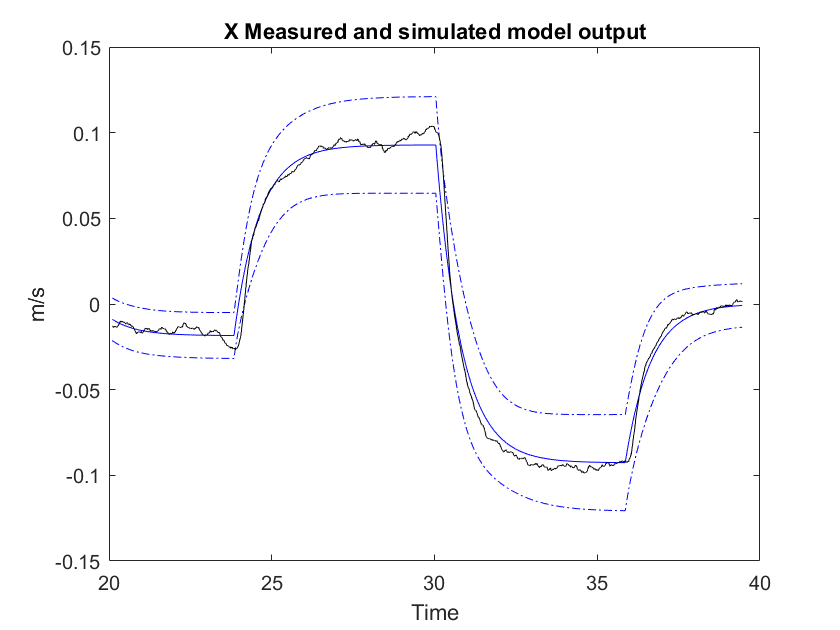
\includegraphics[width=0.7\textwidth]{figs/chapter4/valxtimeplot.png}
    \caption{Confronto tra l'output misurato e quello approssimato (in blu) sul validation set dell'asse $x$. In tratteggio l'intervallo di confidenza.}
    \label{fig:xvalerr}
\end{figure}

\begin{figure}
    \centering
    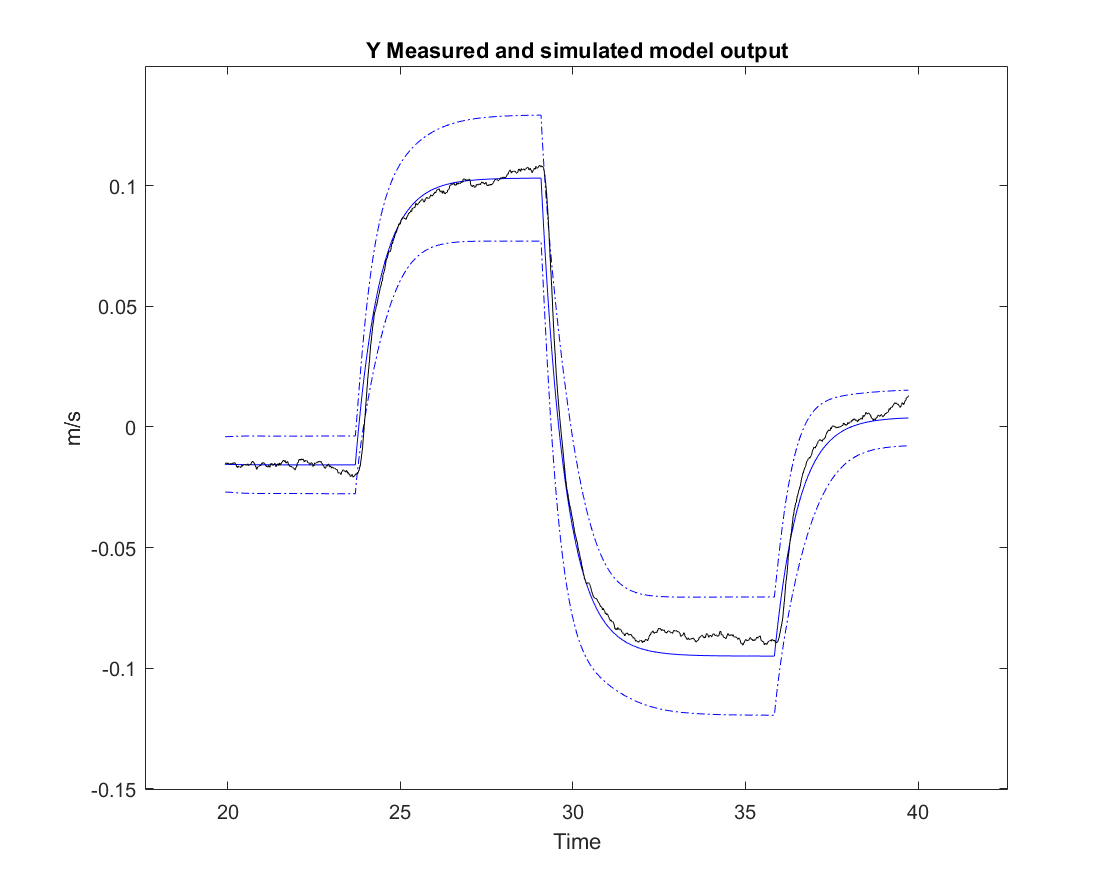
\includegraphics[width=0.7\textwidth]{figs/chapter4/valytimeplot.png}
    \caption{Confronto tra l'output misurato e quello approssimato (in blu) sul validation set dell'asse $y$. In tratteggio l'intervallo di confidenza.}
    \label{fig:yvalerr}
\end{figure}

\newsection{Design del controllore}
\indent La prima soluzione ad essere stata pensata per il problema del precision landing consisteva in un controllore PID da tarare opportunamente mediante esperimenti. Un suo schema ideale è mostrato in Figura \ref{fig:nspid}. Al di là dei problemi tecnici riscontrati con la camera inferiore nella realtà questa soluzione non assicurava performance ottimali, anche per via del tempo di campionamento abbastanza elevato.\\
In questo capitolo, nel nuovo contesto posto dalla definizione del problema, si propone una soluzione alternativa basata sulla seguente idea: iniziare a caricare l'integrale solo a regime. Tale costruzione è stata adeguatamente descritta in \cite{pisw}, e conferisce al sistema di controllo la caratteristica di essere \emph{switching}, rientrando in una classe più complessa e nonlineare ma le cui prestazioni sono in genere migliori delle controparti lineari. Un diagramma riassuntivo del controllore progettato applicato al sistema da controllare è mostrato in Figura \ref{fig:swpi}: si noti in particolare come il sistema sia stato modellato come una serie tra il modello identificato e un puro integratore della sua uscita, per ottenere la posizione lungo l'asse corrente restituita da PX4 sulla base della quale è calcolato l'errore pubblicato dall'Aruco Scanner.\\
La principale differenza di questo schema rispetto a un classico PI è la presenza di una commutazione internamente al blocco integratore: ad ogni istante di tempo il guadagno $k_i$ del termine integrale può assumere uno tra due possibili valori: pari ad un guadagno costante opportunamente scelto o ad un coefficiente molto piccolo. La selezione di tali differenti guadagni dipende dallo stato del sistema d'errore che qui viene approssimato al secondo ordine, ($e$, $\dot e$), nelle rispettive coordinate $x$ ed $y$. È in questo che risiede la peculiarità di tale controllore, in quanto appunto switching: si tratta di un sistema dinamico nonlineare che integra al suo interno due dinamiche, la prima a tempo continuo corrispondente a quella di un PI e la seconda a tempo discreto, la quale ad ogni istante decide se commutare il guadagno del termine integrale da quello corrente all'altro. Volendo riassumere la teoria descritta in \cite{pisw} supponiamo di disporre, come in questo caso è, di una misura del segnale d'errore $e(t)$. Definiamo pertanto il seguente funzionale di costo $J$:
\begin{equation}
    J(t) = \int_{0}^{\infty} (w_1e^2(\tau) + w_2\dot{e}^2(\tau)) \,d\tau
\end{equation}
dove la variabile indipendente $t$ indica un generico istante di commutazione e $w_1, w_2 > 0$. Si può dimostrare che tale funzionale ammette svariati punti di minimo locale. È lecito supporre che il drone sia sufficientemente stabilizzato per poter essere mantenuto a regime una volta raggiunto il target, ipotesi operativa che riporta nelle stesse condizioni del caso di specie trattato in \cite{pisw}. È dunque possibile provare che il problema di controllo si traduce così in quello di determinare, tra tutti i possibili punti di minimo locale di $J(t)$, quello che corrisponde al minimo valore possibile di suddetto funzionale. Sia $t^*$ tale punto, allora per conseguire l'obiettivo di controllo è sufficiente una sola commutazione del guadagno dell'integrale, in modo da iniziare a caricarlo solo una volta che si è raggiunta la condizione di regime, la quale corrisponde ad un box set nel piano $(e, \dot{e})$ che indica una situazione in cui il drone è sufficientemente vicino al target e sta iniziando ad assestarsi in sua prossimità; una rappresentazione esplicativa di tale insieme è offerta in Figura \ref{fig:ebox}. Infine, un altro problema da risolvere riguarda il calcolo della derivata del segnale d'errore, ossia $\dot{e}(t)$. Essendo in presenza di un sistema di controllo evidentemente a tempo discreto in quanto operante sulla base di segnali campionati a frequenze fissate, nel presente lavoro è stato impiegato un algoritmo iterativo che calcola una derivata numericamente approssimata come un rapporto incrementale, i cui estremi corrispondono alle medie campionarie valutate su due finestre poste all'inizio ed alla fine di un buffer circolare di campioni. Le dimensioni del buffer e delle finestre sono state decise in base alle seguenti osservazioni:
\begin{itemize}
    \item il buffer deve essere sufficientemente ampio da poter osservare variazioni significative del segnale, dunque se la costante di tempo del sistema che lo genera è pari a $\tau$ ed il tempo di campionamento è $T_s$, la dimensione deve essere sufficientemente maggiore di $\frac{\tau}{T_s}$;
    \item data la dimensione del buffer, le finestre devono essere ampie quanto basta affinché i loro centri distino temporalmente di un quantitativo comparabile a $\tau$.
\end{itemize}
Il design del controllore è stato eseguito in Simulink per ciascuno dei due sistemi identificati, implementandolo in codice MATLAB comprensivo di opportune saturazioni della variabile di controllo, pari alle reali impostazioni eseguite su PX4 che limitano le velocità lineari in ogni modalità ad un'ampiezza massima di 0.5 m/s. Lo schema impiegato per il design e la taratura su ciascun asse prevede due sistemi da controllare identici ma soggetti l'uno all'azione del PI switching, l'altro a quella di un PI discretizzato tarato automaticamente da Simulink stesso. A titolo d'esempio si riporta in Figura \ref{fig:compmodel} il modello costruito per l'asse $y$. Si noti in esso l'aggiunta del disturbo costante approssimante il vento sul ramo d'ingresso del sistema identificato, puramente per necessità implementative nella simulazione su Gazebo.\\
La simulazione è stata impostata posizionando inizialmente il sistema a 2 metri dal target. I risultati migliori con il controllore PI switching sono stati ottenuti su entrambi gli assi in corrispondenza dei parametri riportati nella Tabella \ref{tab:cparams}. I risultati delle simulazioni con tali parametri sono presentati nelle Figure \ref{fig:xcomp} e \ref{fig:ycomp}. Da essi si evince come le performance nel transitorio del controllore switching siano nettamente superiori a quelle della controparte standard: l'inserimento a regime dell'azione integrale evita del tutto le sovraelongazioni e le oscillazioni intorno al valore di regime, consentendo di raggiungere quest'ultimo poco dopo il tempo di salita, pari a circa 6 secondi. Durante la salita il segnale di controllo generato da entrambe le soluzioni satura immediatamente: ciò impedisce di velocizzare la risposta alzando il guadagno del termine proporzionale, o aggiungendo uno switch anche su di esso. Di contro, nella realtà tali saturazioni sono necessarie per evitare movimenti troppo bruschi compiuti dal drone in caso di problemi in questo o in altri punti dell'architettura, e sono state considerate anche in questa simulazione al fine di renderla il più possibile significativa.

\begin{table}
    \centering
    \begin{tabular}{c|c}
        $k_p$ & 0.9 \\
        $k_i$ & 0.3 \\
        $\sigma_e$ & 0.2 m\\
        $\sigma_{de}$ & 0.1 m/s\\
        $\sigma_{u}$ & 0.5 m/s\\
        Dimensione buffer & 16 campioni\\
        Dimensione finestre & 5 campioni
    \end{tabular}
    \caption{Parametri di funzionamento ottimali dei controllori PI switching.}
    \label{tab:cparams}
\end{table}

\begin{figure}
    \begin{center}
        \begin{tikzpicture}[auto, node distance=1cm, >=latex']
            % Blocks
            \node (ref) [input] {};
            \node (sume) [sum, right=of ref] {};
            \node (dote) [coordinate, right=of sume] {};
            \node (i) [block, right=of dote] {$\int_{0}^{t} k_ie(\tau) \,d\tau$};
            \node (p) [block, above=of i] {$k_pe(t)$};
            \node (d) [block, below=of i] {$k_d\frac{de(t)}{dt}$};
            \node (sumc) [sum, right=of i] {};
            \node (plant) [block, right=of sumc] {P};
            \node (doty) [coordinate, right=of plant] {};
            \node (output) [output, right=of doty] {};
            % Connections
            \draw [->] (ref)  -- node {$r$} node[pos=0.7, below] {$+$} (sume);
            \draw [-] (sume) -- node {$e$} (dote);
            \draw [->] (dote) |- node {} (p);
            \draw [->] (dote) -- node {} (i);
            \draw [->] (dote) |- node {} (d);
            \draw [->] (p) -| node[pos=0.2] {$u_p$} node[pos=0.95, right] {$+$} (sumc);
            \draw [->] (i) -- node {$u_i$} node[pos=0.8, below] {$+$} (sumc);
            \draw [->] (d) -| node[pos=0.2, above] {$u_d$} node[pos=0.95, right] {$+$} (sumc);
            \draw [->] (sumc) -- node {$u$} (plant);
            \draw [->] (plant) -- node {$y$} (output);
            \draw [->] (doty) -- ++ (0,-3.5) -| node[pos=0.95, right] {$-$} (sume);
        \end{tikzpicture}
        \caption{Diagramma a blocchi di un controllore PID ideale.}
        \label{fig:nspid}
    \end{center}
\end{figure}

\begin{figure}
    \begin{center}
        \begin{tikzpicture}[auto, node distance=0.8cm, >=latex']
            % Blocks
            \node (ref) [input] {};
            \node (sume) [sum, right=of ref] {};
            \node (dote) [coordinate, right=of sume] {};
            \node (i) [block, right=of dote] {$\int_{0}^{t} k_ie(\tau) \,d\tau$};
            \node (p) [block, above=of i] {$k_pe(t)$};
            \node (sumc) [sum, right=of i] {};
            \node (plant) [block, right=of sumc] {Identified model};
            \node (integ) [block, right=of plant] {$\int_{0}^{t} v(\tau) \,d\tau$};
            \node (dotp) [coordinate, right=of integ] {};
            \node (output) [output, right=of dotp] {};
            % Connections
            \draw [->] (ref)  -- node {$r$} node[pos=0.7, below] {$+$} (sume);
            \draw [-] (sume) -- node {$e$} (dote);
            \draw [->] (dote) |- node {} (p);
            \draw [->] (dote) -- node {} (i);
            \draw [->] (p) -| node[pos=0.2] {$u_p$} node[pos=0.95, right] {$+$} (sumc);
            \draw [->] (i) -- node {$u_i$} node[pos=0.8, below] {$+$} (sumc);
            \draw [->] (sumc) -- node {$u$} (plant);
            \draw [->] (plant) -- node {$v$} (integ);
            \draw [->] (integ) -- node {$p$} (output);
            \draw [->] (dotp) -- ++ (0,-2) -| node[pos=0.95, right] {$-$} (sume);
        \end{tikzpicture}
        \caption{Diagramma a blocchi del sistema di controllo sviluppato.}
        \label{fig:swpi}
    \end{center}
\end{figure}

\begin{figure}
    \centering
    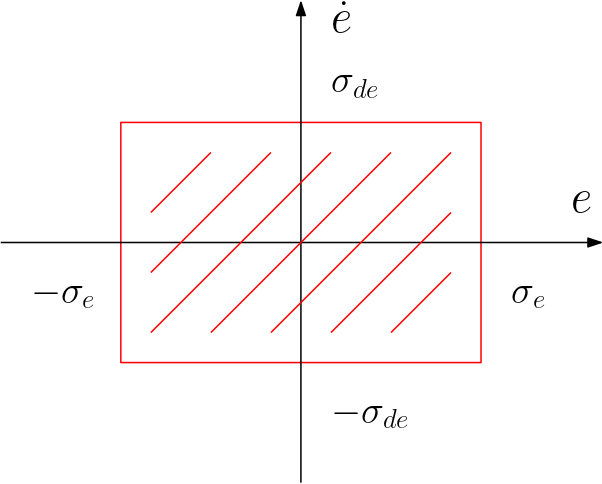
\includegraphics[width=0.6\textwidth]{figs/chapter4/ebox.png}
    \caption{Box set rappresentante la condizione di regime nel piano $(e, \dot{e})$.}
    \label{fig:ebox}
\end{figure}

\begin{figure}
    \centering
    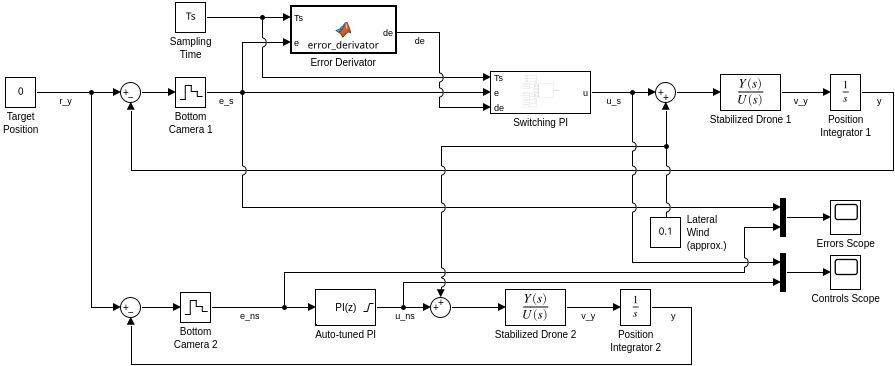
\includegraphics[width=\textwidth]{figs/chapter4/compmodel.jpg}
    \caption{Modello impiegato per il design del controllore relativo all'asse $y$.}
    \label{fig:compmodel}
\end{figure}

\begin{figure}
    \centering
    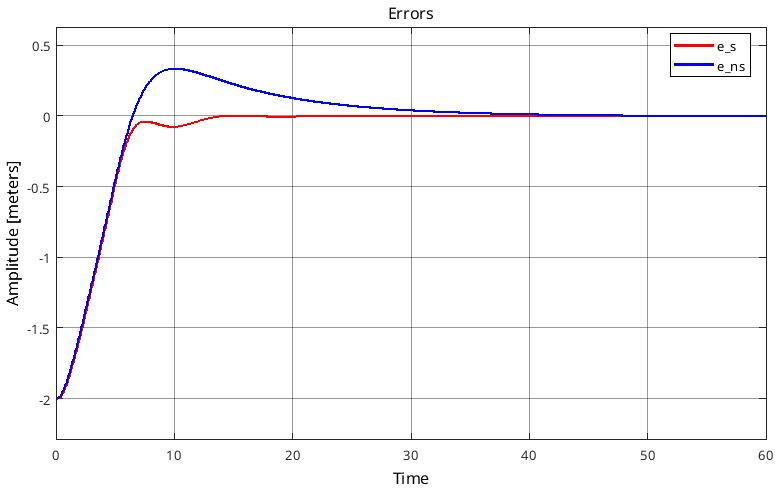
\includegraphics[width=\textwidth]{figs/chapter4/xerrcomp.jpg}
    \vspace{0.2cm}
    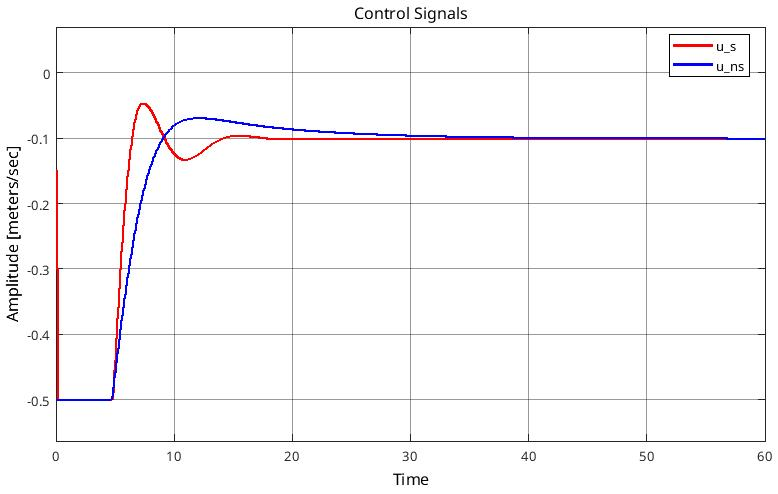
\includegraphics[width=\textwidth]{figs/chapter4/xcontrolcomp.jpg}
    \caption{Confronto tra l'andamento dell'errore e del segnale di controllo generati dal controllore PI switching (rosso) e non-switching (blu) per l'asse $x$.}
    \label{fig:xcomp}
\end{figure}

\begin{figure}
    \centering
    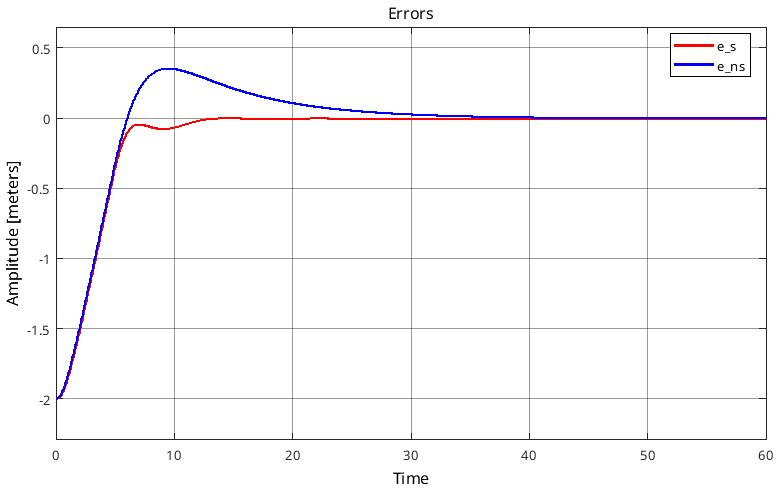
\includegraphics[width=\textwidth]{figs/chapter4/yerrcomp.jpg}
    \vspace{0.2cm}
    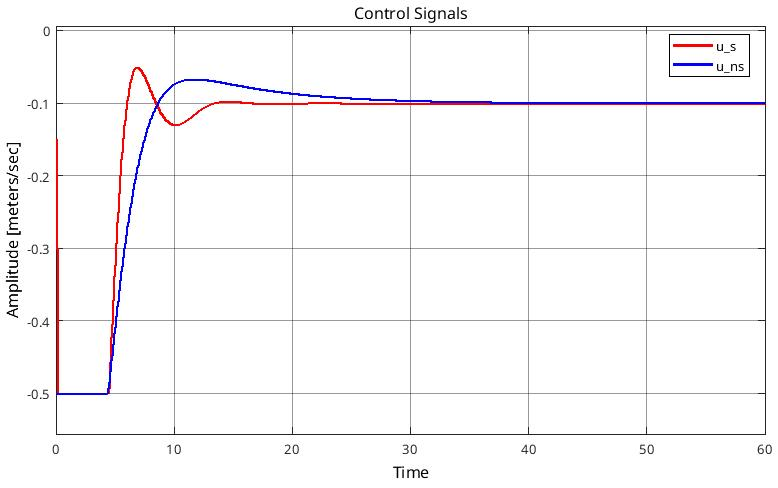
\includegraphics[width=\textwidth]{figs/chapter4/ycontrolcomp.jpg}
    \caption{Confronto tra l'andamento dell'errore e del segnale di controllo generati dal controllore PI switching (rosso) e non-switching (blu) per l'asse $y$.}
    \label{fig:ycomp}
\end{figure}
\clearpage

\newsection{Implementazione in ROS 2}
\indent Il confronto effettuato nella sezione precedente è stato ripetuto in Gazebo. L'implementazione del PI non-switching era già stata realizzata ed è stata pertanto riadattata cambiando i guadagni, posti pari a quelli risultati ottimali per la versione switching. Quest'ultima ed i derivatori numerici sono stati invece implementati in C++ come classi, ed impiegati in una nuova callback dal topic /ArucoErrors con cui è stato compilato un nuovo eseguibile del package precision\_landing, denominato \emph{switching\_pi}. Disponendo già del resto dell'architettura, nonché del codice del nodo precision\_landing in cui integrare immediatamente la nuova callback, l'implementazione dei nuovi controllori ha richiesto uno sforzo molto contenuto. La simulazione in Gazebo è stata effettuata portando il drone a 2 metri di quota al di sopra di una replica della piazzola 1, applicando un vento trasversale con contributi sia sull'asse $x$ che sull'asse $y$, e richiedendo il precision landing tramite l'apposito servizio. La posizione iniziale era la stessa a meno di minime oscillazioni del drone posto in hovering. I risultati sono riportati in Figura \ref{fig:gazcomp}. Si nota immediatamente il passaggio al modello nonlineare: sono infatti presenti delle minime oscillazioni nel tracciato relativo al controllore switching. Esso porta comunque a termine l'allineamento in breve tempo, a seguito del quale viene richiesto l'atterraggio al Flight Control. La cosa che più salta agli occhi però è l'incapacità del controllore PI non-switching, implementato con gli stessi guadagni della controparte, di eseguire l'allineamento: nonostante ripetuti tentativi, di cui quello mostrato è uno, le oscillazioni indotte dal termine integrale erano eccessive e portavano la camera inferiore a perdere il target, situazione dalla quale la logica di supervisione usciva facendo fallire la procedura dopo un timeout come previsto. Questa simulazione, nonostante sia puramente indicativa, porta comunque a delle conclusioni interessanti: innanzitutto si è dimostrato come su un'architettura di controllo basata su ROS 2 sia stato possibile implementare efficacemente sistemi di controllo anche complessi, come appunto dei PI switching, e poi si è reso evidente come la classe dei controllori switching, anche nelle versioni più semplici, consenta di ottenere delle performance di molto migliori delle controparti non-switching anche in contesti problematici come quello in esame, caratterizzato da un elevato tempo di campionamento del segnale d'errore e da una notevole approssimazione del modello del sistema da controllare.

\begin{figure}
    \centering
    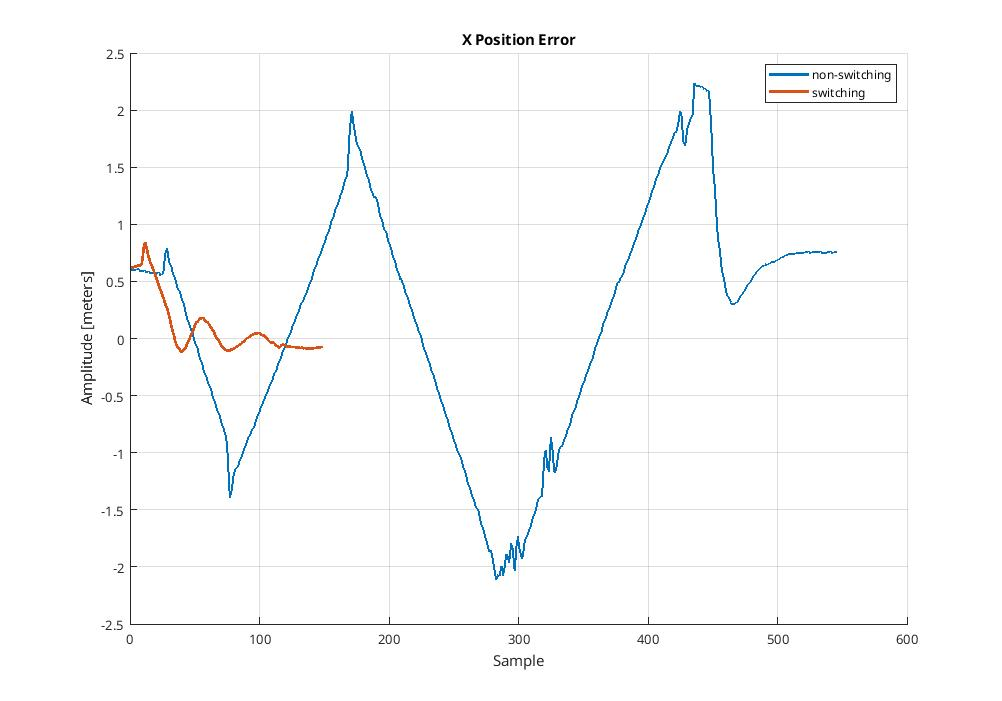
\includegraphics[scale=0.4]{figs/chapter4/xgaz.jpg}
    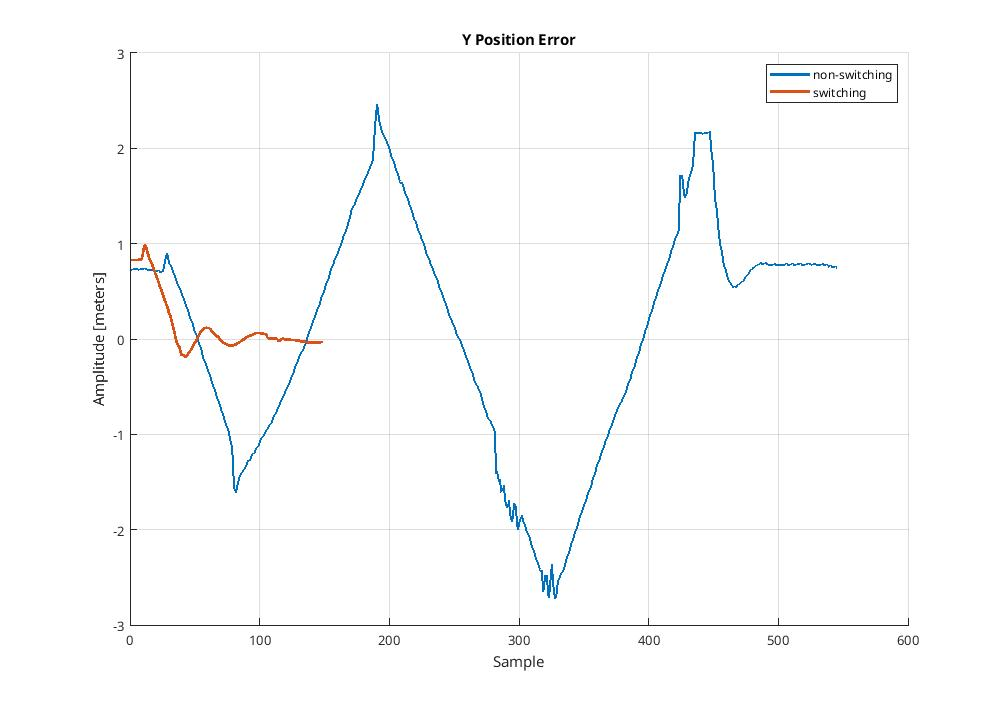
\includegraphics[scale=0.4]{figs/chapter4/ygaz.jpg}
    \caption{Andamento dell'errore indotto dai controllori PI switching (rosso) e non-switching (blu) durante un precision landing in Gazebo.}
    \label{fig:gazcomp}
\end{figure}
